% This LaTeX was auto-generated from MATLAB code.
% To make changes, update the MATLAB code and export to LaTeX again.

\documentclass{article}

\usepackage[utf8]{inputenc}
\usepackage[T1]{fontenc}
\usepackage{lmodern}
\usepackage{graphicx}
\usepackage{color}
\usepackage{hyperref}
\usepackage{amsmath}
\usepackage{amsfonts}
\usepackage{epstopdf}
\usepackage[table]{xcolor}
\usepackage{matlab}

\sloppy
\epstopdfsetup{outdir=./}
\graphicspath{ {./Laboratorio_3_images/} }

\begin{document}

\matlabtitle{Atividade de laboratório }

\matlabheading{Redimensionamento de imagens}

\begin{matlabcode}
%Carrega a imagem
x = imread("Lenna.jpg");
imshow(x, 'InitialMagnification',100);
\end{matlabcode}
\begin{center}
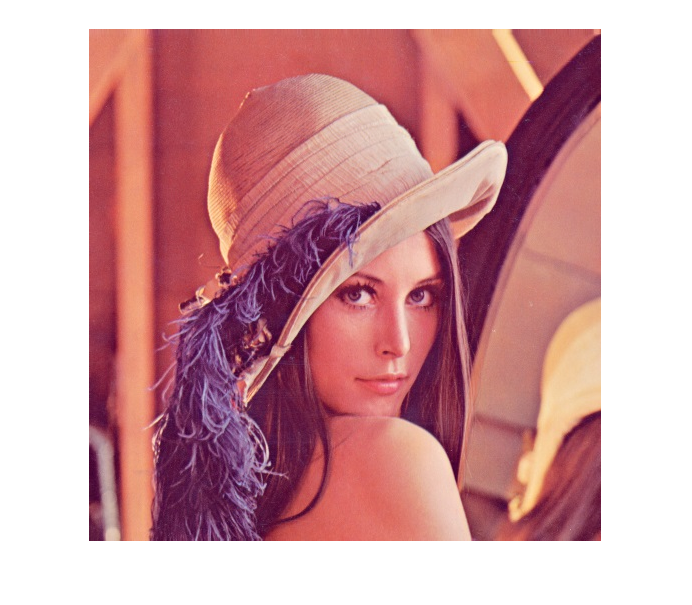
\includegraphics[width=\maxwidth{69.44305067737079em}]{figure_0.png}
\end{center}
\begin{matlabcode}

%Converte para escala de cinza
x_cinza = rgb2gray(x);
%Normaliza
x_cinza = double(x_cinza)/255;
%Mostra a imagem com o tamanho correto para ser possivel ver alteracao de
%tamanho
imshow(x_cinza,'InitialMagnification',100);
\end{matlabcode}
\begin{center}
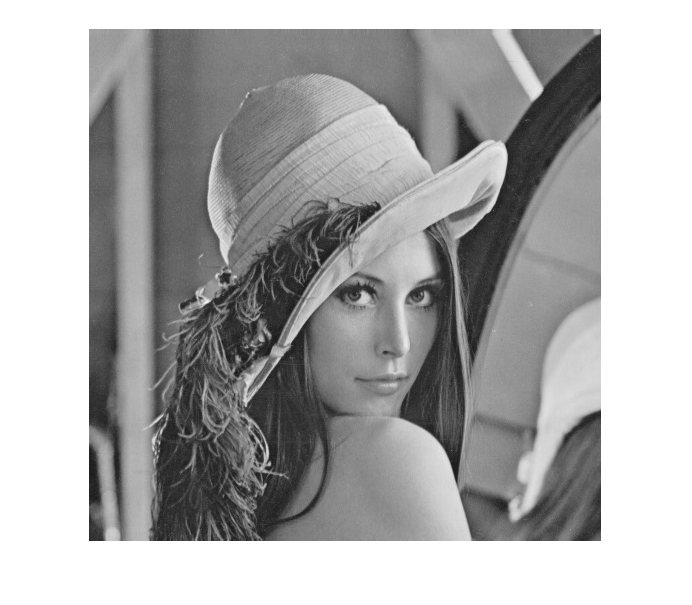
\includegraphics[width=\maxwidth{69.44305067737079em}]{figure_1.png}
\end{center}
\begin{matlabcode}

%Mostra a imagem com tamanho comprimido
y_comprimido = dil_or_com(x_cinza,"c");
imshow(y_comprimido,'InitialMagnification',100);
\end{matlabcode}
\begin{center}
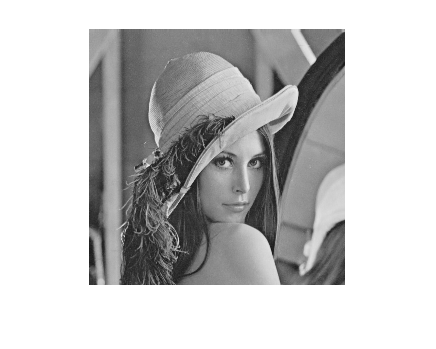
\includegraphics[width=\maxwidth{43.753135975915704em}]{figure_2.png}
\end{center}
\begin{matlabcode}


%Mostra a imagem com tamanho dilatado
y_dilatado = dil_or_com(x_cinza,"d");
imshow(y_dilatado, 'InitialMagnification',100);
\end{matlabcode}
\begin{center}
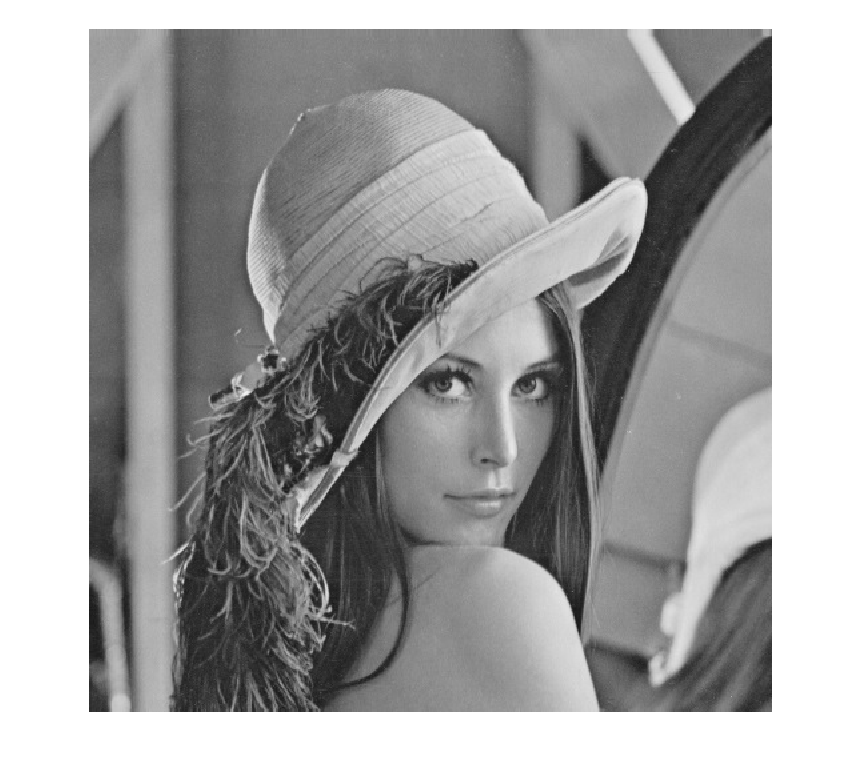
\includegraphics[width=\maxwidth{85.39889613647767em}]{figure_3.png}
\end{center}
\begin{matlabcode}

\end{matlabcode}

\matlabheading{Quantizaçao de Imagens}

\begin{matlabcode}
x = imread("Lenna.jpg");
imshow(x);
\end{matlabcode}
\begin{center}
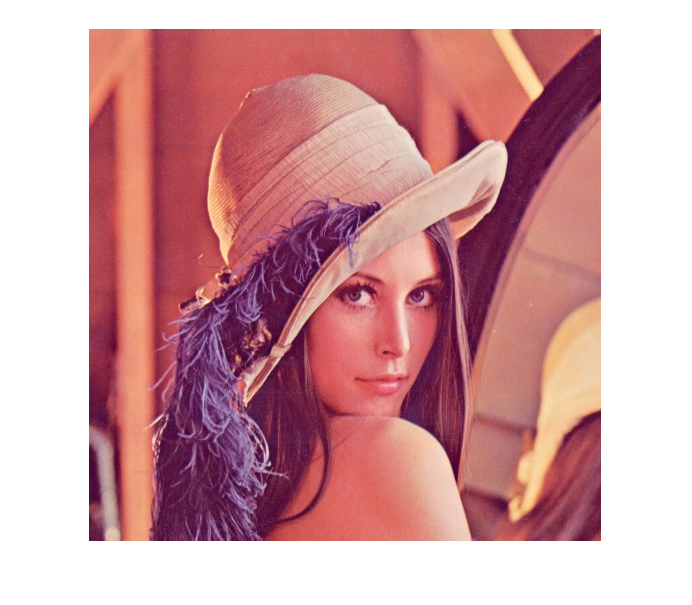
\includegraphics[width=\maxwidth{69.44305067737079em}]{figure_4.png}
\end{center}
\begin{matlabcode}

%Converte para escala de cinza e normaliza
x = double(rgb2gray(x))/255;
imshow(x);
\end{matlabcode}
\begin{center}
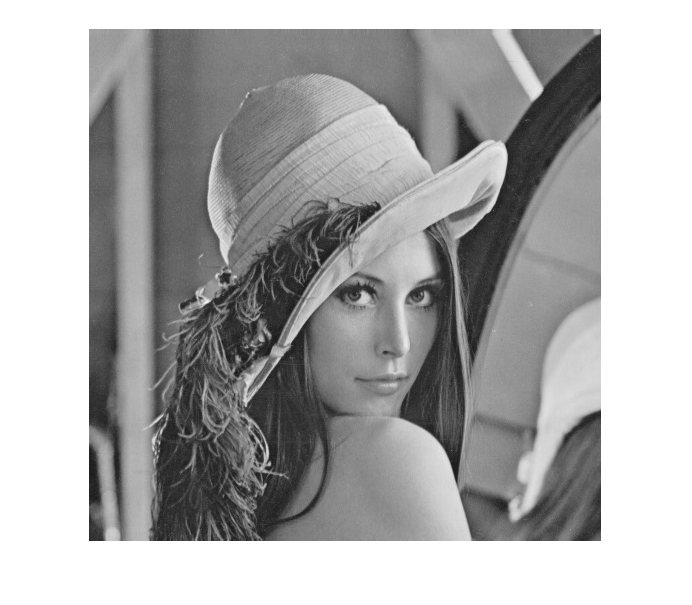
\includegraphics[width=\maxwidth{69.44305067737079em}]{figure_5.png}
\end{center}
\begin{matlabcode}
plot_quantizacao(x);
\end{matlabcode}
\begin{center}
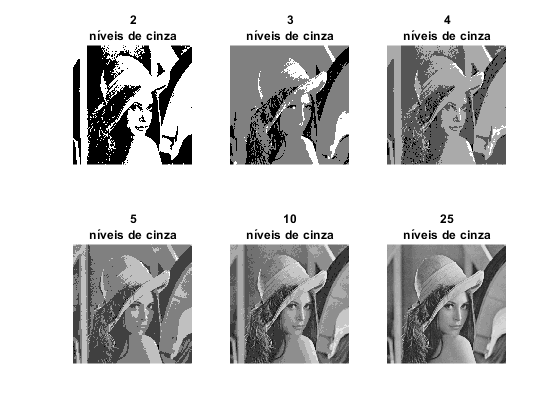
\includegraphics[width=\maxwidth{56.196688409433015em}]{figure_6.png}
\end{center}
\begin{matlabcode}
plot_erro_relativo(x);
\end{matlabcode}
\begin{center}
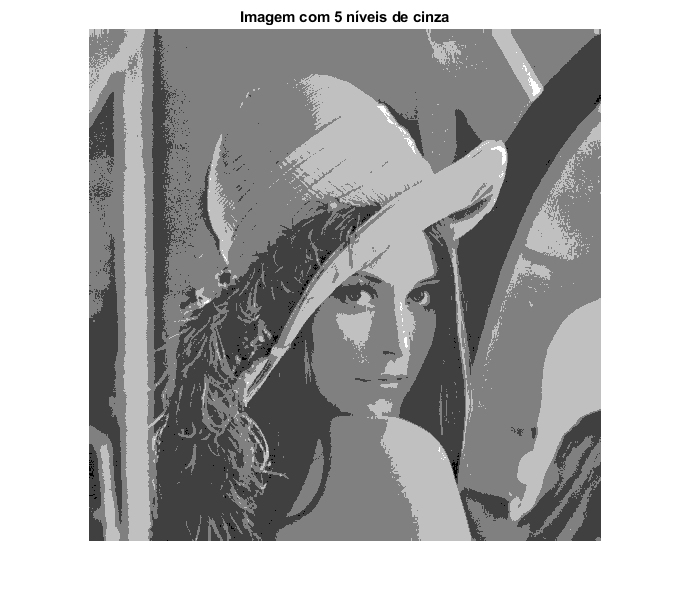
\includegraphics[width=\maxwidth{56.196688409433015em}]{figure_7.eps}
\end{center}
\begin{matlabcode}
x = imread("galaxy.jpeg");
imshow(x);
\end{matlabcode}
\begin{center}
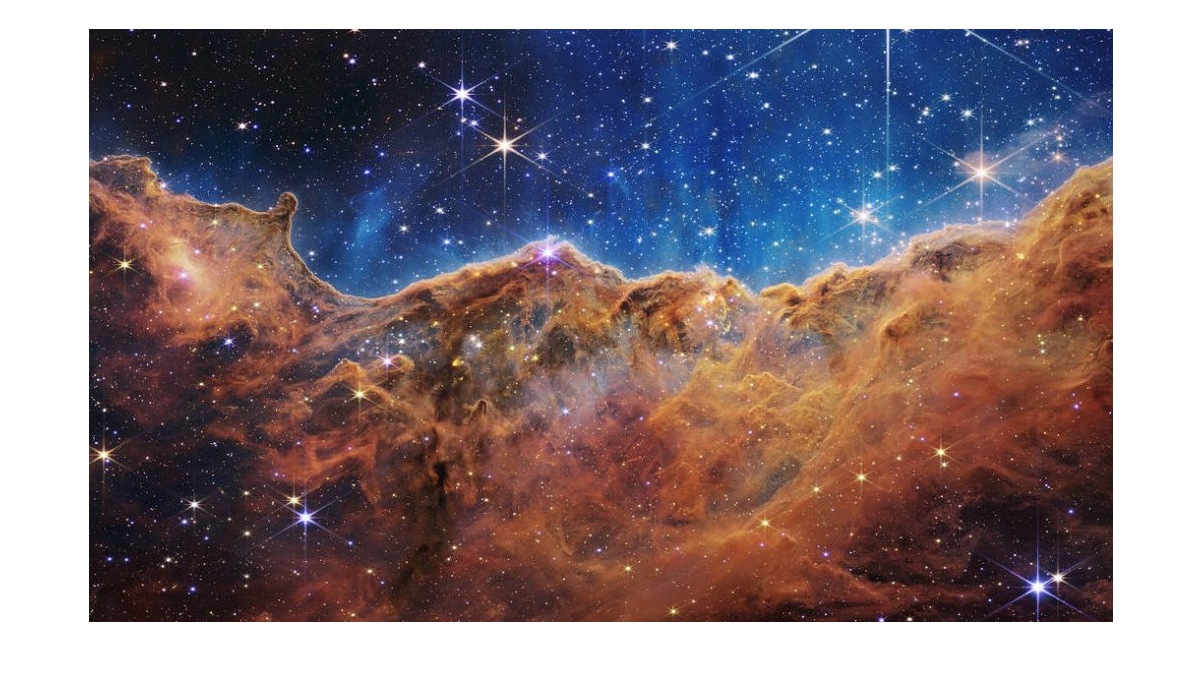
\includegraphics[width=\maxwidth{85.39889613647767em}]{figure_8.png}
\end{center}
\begin{matlabcode}
%Converte para escala de cinza e normaliza
x = double(rgb2gray(x))/255;
imshow(x);
\end{matlabcode}
\begin{center}
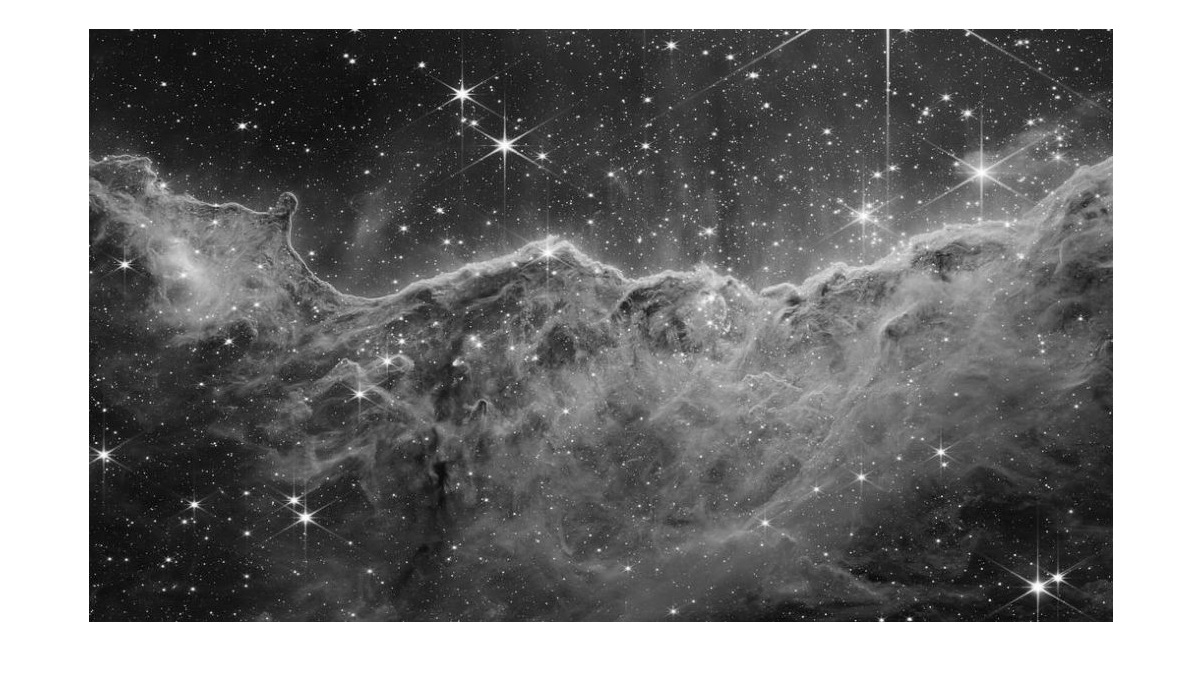
\includegraphics[width=\maxwidth{85.39889613647767em}]{figure_9.png}
\end{center}
\begin{matlabcode}

plot_quantizacao(x);
\end{matlabcode}
\begin{center}
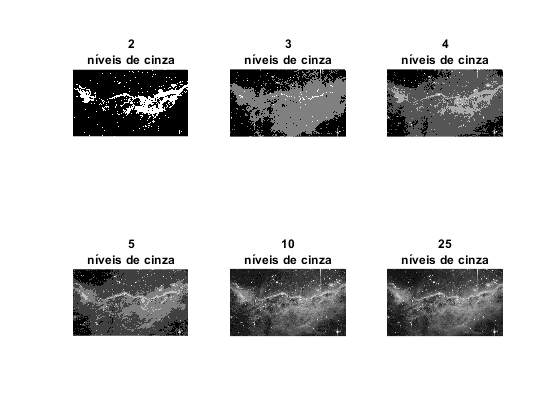
\includegraphics[width=\maxwidth{56.196688409433015em}]{figure_10.png}
\end{center}
\begin{matlabcode}
plot_erro_relativo(x);
\end{matlabcode}
\begin{center}
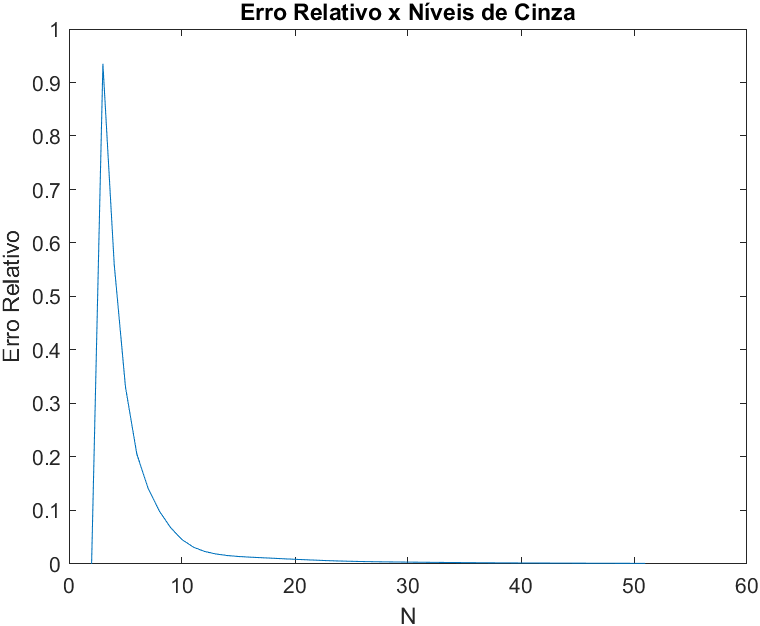
\includegraphics[width=\maxwidth{56.196688409433015em}]{figure_11.eps}
\end{center}
\begin{matlabcode}
x = imread("olho.jpg");
figure;
imshow(x);
\end{matlabcode}
\begin{center}
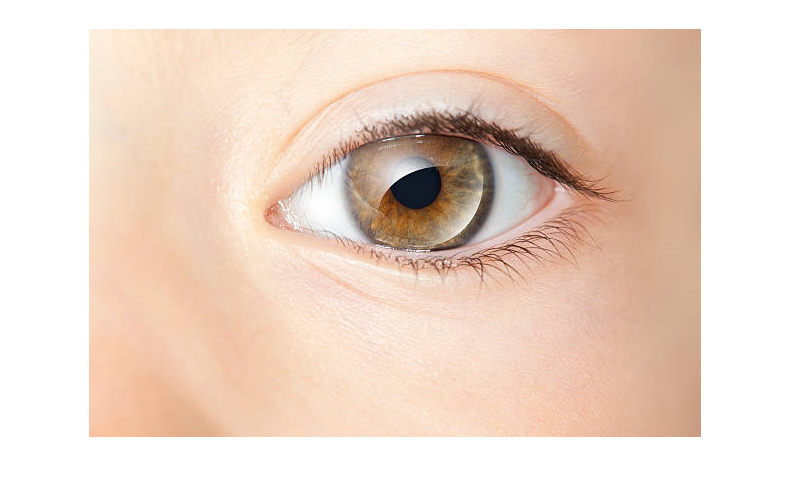
\includegraphics[width=\maxwidth{79.4781736076267em}]{figure_12.png}
\end{center}
\begin{matlabcode}
%Converte para escala de cinza e normaliza
x = double(rgb2gray(x))/255;
imshow(x);
\end{matlabcode}
\begin{center}
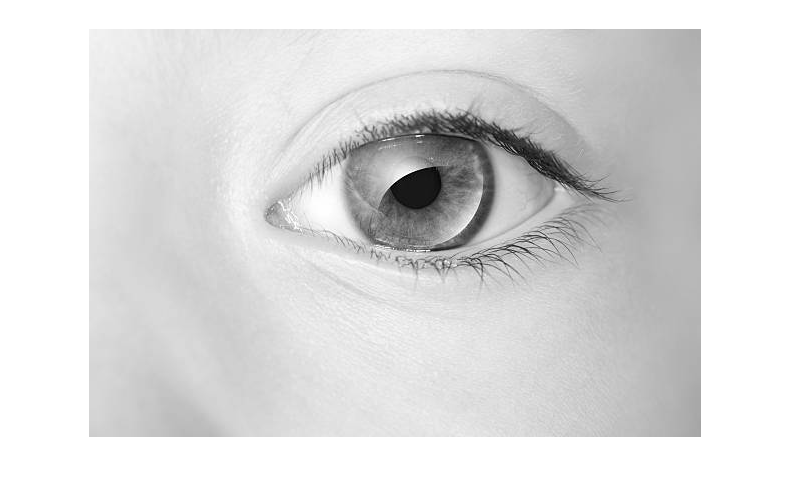
\includegraphics[width=\maxwidth{79.4781736076267em}]{figure_13.png}
\end{center}
\begin{matlabcode}

plot_quantizacao(x);
\end{matlabcode}
\begin{center}
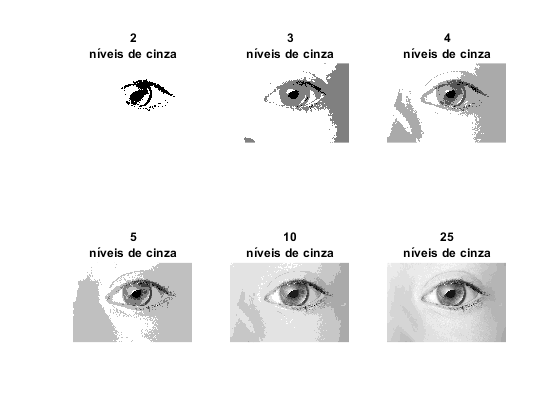
\includegraphics[width=\maxwidth{56.196688409433015em}]{figure_14.png}
\end{center}
\begin{matlabcode}
plot_erro_relativo(x);
\end{matlabcode}
\begin{center}
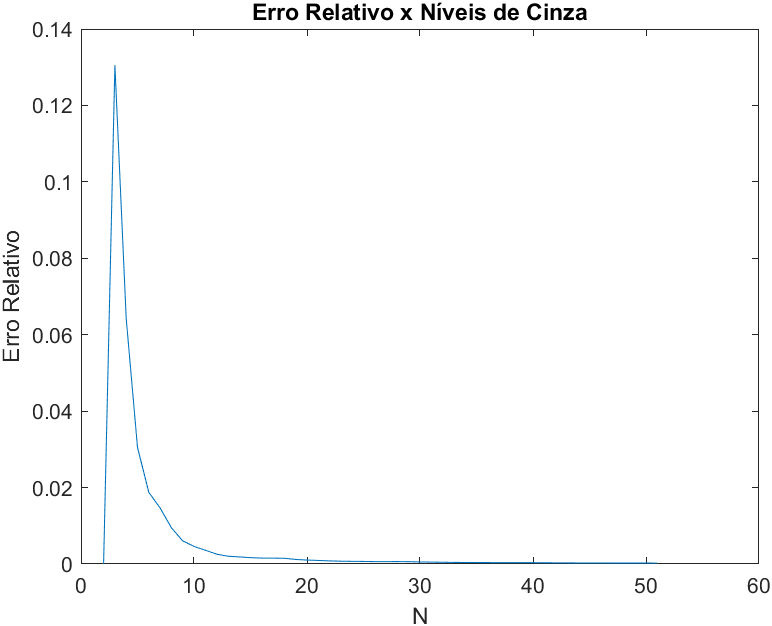
\includegraphics[width=\maxwidth{56.196688409433015em}]{figure_15.eps}
\end{center}

\begin{par}
\begin{flushleft}
Através dos testes de quantização utilizando varios tipos de niveis de cinza foi possivel notar que quanto maior a quantidade de niveis de cinza, mais nítida é a imagem e isso também implica que o erro relativo é menor para niveis de cinza suficientemente grandes, por exemplo: com N igual a 25 ja foi possivel observar que a imagem estava bem nítida, porém não tanto quanto a originial pois ao fundo é possível perceber pequenos 'borrões'.
\end{flushleft}
\end{par}

\matlabheading{Funções Utilizadas}


\begin{matlabcode}
function y = dil_or_com (x,modo)
    [L,C] = size(x);
    %Parte que faz a dilatação
    if(modo == 'd')
        x_dil = zeros(L*2,C*2);
        for i = 1 : L
            for j = 1 : C
                atual = x(i,j);
                x_dil(i+i-1,j+j-1) = atual;
                x_dil(i+i-1+1,j+j-1) = atual;
                x_dil(i+i-1,j+j-1+1) = atual;
                x_dil(i+i-1+1,j+j-1+1) = atual;
            end
        end
        y = x_dil;
   %Parte que faz a compressão 
    else 
        if (modo == 'c')
            [L,C] = size(x);
            x_com = zeros(round(L/2),round(C/2));
            [L,C] = size(x_com);
            for i = 1 : L
                for j = 1 : C
                    atual = x(i+i-1,j+j-1);
                    x_com(i,j) = atual;
                    x_com(i+1,j) = atual;
                    x_com(i,j+1) = atual;
                    x_com(i+1,j+1) = atual;
                end
            end
            %Deixando do tamanho correto pois estava gerando uma linha e uma coluna
            %extra
            x_com = x_com(1:end-1, 1:end-1);
            y = x_com;
        end
    end
end
    
function [y, erro_relativo] = quantizacao (x,N)
    niveis = linspace(0,1,N);
    y = interp1(niveis, niveis, x, 'nearest');
    [L,C] = size(x);
    num = zeros(L,C);
    den = num;
    for i = 1 : L
        for j = 1 : C
            num(i,j) = (abs(x(i,j) - y(i,j)))^2;
            den(i,j) = (abs(x(i,j)))^2;
        end
    end
    erro_relativo = num./(den+eps);
    erro_relativo = mean(erro_relativo(:));
end
function plot_erro_relativo(x)
    vet_N = 2:256;
    vet_erros = zeros(1,255);
    for N = 2 : length(vet_N)
        [y, vet_erros(N)] = quantizacao(x,N);
    end
    figure;
    plot(vet_N(1:50),vet_erros(1:50));
    xlabel('N');
    ylabel('Erro Relativo');
    title('Erro Relativo x Níveis de Cinza');
end

function plot_quantizacao(x)
    vet_N = [2 3 4 5 10 25];
    figure;
    for i = 1 : 6
        [y,z] = quantizacao(x,vet_N(i));
        subplot(2,3,i);
        imshow(y);
        title([int2str(vet_N(i)),"níveis de cinza"]);
    end
    figure;
end
\end{matlabcode}

\end{document}
